
\documentclass{article} % For LaTeX2e
\usepackage{iclr2024_conference,times}

% Optional math commands from https://github.com/goodfeli/dlbook_notation.
%%%%% NEW MATH DEFINITIONS %%%%%

\usepackage{amsmath,amsfonts,bm}

% Mark sections of captions for referring to divisions of figures
\newcommand{\figleft}{{\em (Left)}}
\newcommand{\figcenter}{{\em (Center)}}
\newcommand{\figright}{{\em (Right)}}
\newcommand{\figtop}{{\em (Top)}}
\newcommand{\figbottom}{{\em (Bottom)}}
\newcommand{\captiona}{{\em (a)}}
\newcommand{\captionb}{{\em (b)}}
\newcommand{\captionc}{{\em (c)}}
\newcommand{\captiond}{{\em (d)}}

% Highlight a newly defined term
\newcommand{\newterm}[1]{{\bf #1}}


% Figure reference, lower-case.
\def\figref#1{figure~\ref{#1}}
% Figure reference, capital. For start of sentence
\def\Figref#1{Figure~\ref{#1}}
\def\twofigref#1#2{figures \ref{#1} and \ref{#2}}
\def\quadfigref#1#2#3#4{figures \ref{#1}, \ref{#2}, \ref{#3} and \ref{#4}}
% Section reference, lower-case.
\def\secref#1{section~\ref{#1}}
% Section reference, capital.
\def\Secref#1{Section~\ref{#1}}
% Reference to two sections.
\def\twosecrefs#1#2{sections \ref{#1} and \ref{#2}}
% Reference to three sections.
\def\secrefs#1#2#3{sections \ref{#1}, \ref{#2} and \ref{#3}}
% Reference to an equation, lower-case.
\def\eqref#1{equation~\ref{#1}}
% Reference to an equation, upper case
\def\Eqref#1{Equation~\ref{#1}}
% A raw reference to an equation---avoid using if possible
\def\plaineqref#1{\ref{#1}}
% Reference to a chapter, lower-case.
\def\chapref#1{chapter~\ref{#1}}
% Reference to an equation, upper case.
\def\Chapref#1{Chapter~\ref{#1}}
% Reference to a range of chapters
\def\rangechapref#1#2{chapters\ref{#1}--\ref{#2}}
% Reference to an algorithm, lower-case.
\def\algref#1{algorithm~\ref{#1}}
% Reference to an algorithm, upper case.
\def\Algref#1{Algorithm~\ref{#1}}
\def\twoalgref#1#2{algorithms \ref{#1} and \ref{#2}}
\def\Twoalgref#1#2{Algorithms \ref{#1} and \ref{#2}}
% Reference to a part, lower case
\def\partref#1{part~\ref{#1}}
% Reference to a part, upper case
\def\Partref#1{Part~\ref{#1}}
\def\twopartref#1#2{parts \ref{#1} and \ref{#2}}

\def\ceil#1{\lceil #1 \rceil}
\def\floor#1{\lfloor #1 \rfloor}
\def\1{\bm{1}}
\newcommand{\train}{\mathcal{D}}
\newcommand{\valid}{\mathcal{D_{\mathrm{valid}}}}
\newcommand{\test}{\mathcal{D_{\mathrm{test}}}}

\def\eps{{\epsilon}}


% Random variables
\def\reta{{\textnormal{$\eta$}}}
\def\ra{{\textnormal{a}}}
\def\rb{{\textnormal{b}}}
\def\rc{{\textnormal{c}}}
\def\rd{{\textnormal{d}}}
\def\re{{\textnormal{e}}}
\def\rf{{\textnormal{f}}}
\def\rg{{\textnormal{g}}}
\def\rh{{\textnormal{h}}}
\def\ri{{\textnormal{i}}}
\def\rj{{\textnormal{j}}}
\def\rk{{\textnormal{k}}}
\def\rl{{\textnormal{l}}}
% rm is already a command, just don't name any random variables m
\def\rn{{\textnormal{n}}}
\def\ro{{\textnormal{o}}}
\def\rp{{\textnormal{p}}}
\def\rq{{\textnormal{q}}}
\def\rr{{\textnormal{r}}}
\def\rs{{\textnormal{s}}}
\def\rt{{\textnormal{t}}}
\def\ru{{\textnormal{u}}}
\def\rv{{\textnormal{v}}}
\def\rw{{\textnormal{w}}}
\def\rx{{\textnormal{x}}}
\def\ry{{\textnormal{y}}}
\def\rz{{\textnormal{z}}}

% Random vectors
\def\rvepsilon{{\mathbf{\epsilon}}}
\def\rvtheta{{\mathbf{\theta}}}
\def\rva{{\mathbf{a}}}
\def\rvb{{\mathbf{b}}}
\def\rvc{{\mathbf{c}}}
\def\rvd{{\mathbf{d}}}
\def\rve{{\mathbf{e}}}
\def\rvf{{\mathbf{f}}}
\def\rvg{{\mathbf{g}}}
\def\rvh{{\mathbf{h}}}
\def\rvu{{\mathbf{i}}}
\def\rvj{{\mathbf{j}}}
\def\rvk{{\mathbf{k}}}
\def\rvl{{\mathbf{l}}}
\def\rvm{{\mathbf{m}}}
\def\rvn{{\mathbf{n}}}
\def\rvo{{\mathbf{o}}}
\def\rvp{{\mathbf{p}}}
\def\rvq{{\mathbf{q}}}
\def\rvr{{\mathbf{r}}}
\def\rvs{{\mathbf{s}}}
\def\rvt{{\mathbf{t}}}
\def\rvu{{\mathbf{u}}}
\def\rvv{{\mathbf{v}}}
\def\rvw{{\mathbf{w}}}
\def\rvx{{\mathbf{x}}}
\def\rvy{{\mathbf{y}}}
\def\rvz{{\mathbf{z}}}

% Elements of random vectors
\def\erva{{\textnormal{a}}}
\def\ervb{{\textnormal{b}}}
\def\ervc{{\textnormal{c}}}
\def\ervd{{\textnormal{d}}}
\def\erve{{\textnormal{e}}}
\def\ervf{{\textnormal{f}}}
\def\ervg{{\textnormal{g}}}
\def\ervh{{\textnormal{h}}}
\def\ervi{{\textnormal{i}}}
\def\ervj{{\textnormal{j}}}
\def\ervk{{\textnormal{k}}}
\def\ervl{{\textnormal{l}}}
\def\ervm{{\textnormal{m}}}
\def\ervn{{\textnormal{n}}}
\def\ervo{{\textnormal{o}}}
\def\ervp{{\textnormal{p}}}
\def\ervq{{\textnormal{q}}}
\def\ervr{{\textnormal{r}}}
\def\ervs{{\textnormal{s}}}
\def\ervt{{\textnormal{t}}}
\def\ervu{{\textnormal{u}}}
\def\ervv{{\textnormal{v}}}
\def\ervw{{\textnormal{w}}}
\def\ervx{{\textnormal{x}}}
\def\ervy{{\textnormal{y}}}
\def\ervz{{\textnormal{z}}}

% Random matrices
\def\rmA{{\mathbf{A}}}
\def\rmB{{\mathbf{B}}}
\def\rmC{{\mathbf{C}}}
\def\rmD{{\mathbf{D}}}
\def\rmE{{\mathbf{E}}}
\def\rmF{{\mathbf{F}}}
\def\rmG{{\mathbf{G}}}
\def\rmH{{\mathbf{H}}}
\def\rmI{{\mathbf{I}}}
\def\rmJ{{\mathbf{J}}}
\def\rmK{{\mathbf{K}}}
\def\rmL{{\mathbf{L}}}
\def\rmM{{\mathbf{M}}}
\def\rmN{{\mathbf{N}}}
\def\rmO{{\mathbf{O}}}
\def\rmP{{\mathbf{P}}}
\def\rmQ{{\mathbf{Q}}}
\def\rmR{{\mathbf{R}}}
\def\rmS{{\mathbf{S}}}
\def\rmT{{\mathbf{T}}}
\def\rmU{{\mathbf{U}}}
\def\rmV{{\mathbf{V}}}
\def\rmW{{\mathbf{W}}}
\def\rmX{{\mathbf{X}}}
\def\rmY{{\mathbf{Y}}}
\def\rmZ{{\mathbf{Z}}}

% Elements of random matrices
\def\ermA{{\textnormal{A}}}
\def\ermB{{\textnormal{B}}}
\def\ermC{{\textnormal{C}}}
\def\ermD{{\textnormal{D}}}
\def\ermE{{\textnormal{E}}}
\def\ermF{{\textnormal{F}}}
\def\ermG{{\textnormal{G}}}
\def\ermH{{\textnormal{H}}}
\def\ermI{{\textnormal{I}}}
\def\ermJ{{\textnormal{J}}}
\def\ermK{{\textnormal{K}}}
\def\ermL{{\textnormal{L}}}
\def\ermM{{\textnormal{M}}}
\def\ermN{{\textnormal{N}}}
\def\ermO{{\textnormal{O}}}
\def\ermP{{\textnormal{P}}}
\def\ermQ{{\textnormal{Q}}}
\def\ermR{{\textnormal{R}}}
\def\ermS{{\textnormal{S}}}
\def\ermT{{\textnormal{T}}}
\def\ermU{{\textnormal{U}}}
\def\ermV{{\textnormal{V}}}
\def\ermW{{\textnormal{W}}}
\def\ermX{{\textnormal{X}}}
\def\ermY{{\textnormal{Y}}}
\def\ermZ{{\textnormal{Z}}}

% Vectors
\def\vzero{{\bm{0}}}
\def\vone{{\bm{1}}}
\def\vmu{{\bm{\mu}}}
\def\vtheta{{\bm{\theta}}}
\def\va{{\bm{a}}}
\def\vb{{\bm{b}}}
\def\vc{{\bm{c}}}
\def\vd{{\bm{d}}}
\def\ve{{\bm{e}}}
\def\vf{{\bm{f}}}
\def\vg{{\bm{g}}}
\def\vh{{\bm{h}}}
\def\vi{{\bm{i}}}
\def\vj{{\bm{j}}}
\def\vk{{\bm{k}}}
\def\vl{{\bm{l}}}
\def\vm{{\bm{m}}}
\def\vn{{\bm{n}}}
\def\vo{{\bm{o}}}
\def\vp{{\bm{p}}}
\def\vq{{\bm{q}}}
\def\vr{{\bm{r}}}
\def\vs{{\bm{s}}}
\def\vt{{\bm{t}}}
\def\vu{{\bm{u}}}
\def\vv{{\bm{v}}}
\def\vw{{\bm{w}}}
\def\vx{{\bm{x}}}
\def\vy{{\bm{y}}}
\def\vz{{\bm{z}}}

% Elements of vectors
\def\evalpha{{\alpha}}
\def\evbeta{{\beta}}
\def\evepsilon{{\epsilon}}
\def\evlambda{{\lambda}}
\def\evomega{{\omega}}
\def\evmu{{\mu}}
\def\evpsi{{\psi}}
\def\evsigma{{\sigma}}
\def\evtheta{{\theta}}
\def\eva{{a}}
\def\evb{{b}}
\def\evc{{c}}
\def\evd{{d}}
\def\eve{{e}}
\def\evf{{f}}
\def\evg{{g}}
\def\evh{{h}}
\def\evi{{i}}
\def\evj{{j}}
\def\evk{{k}}
\def\evl{{l}}
\def\evm{{m}}
\def\evn{{n}}
\def\evo{{o}}
\def\evp{{p}}
\def\evq{{q}}
\def\evr{{r}}
\def\evs{{s}}
\def\evt{{t}}
\def\evu{{u}}
\def\evv{{v}}
\def\evw{{w}}
\def\evx{{x}}
\def\evy{{y}}
\def\evz{{z}}

% Matrix
\def\mA{{\bm{A}}}
\def\mB{{\bm{B}}}
\def\mC{{\bm{C}}}
\def\mD{{\bm{D}}}
\def\mE{{\bm{E}}}
\def\mF{{\bm{F}}}
\def\mG{{\bm{G}}}
\def\mH{{\bm{H}}}
\def\mI{{\bm{I}}}
\def\mJ{{\bm{J}}}
\def\mK{{\bm{K}}}
\def\mL{{\bm{L}}}
\def\mM{{\bm{M}}}
\def\mN{{\bm{N}}}
\def\mO{{\bm{O}}}
\def\mP{{\bm{P}}}
\def\mQ{{\bm{Q}}}
\def\mR{{\bm{R}}}
\def\mS{{\bm{S}}}
\def\mT{{\bm{T}}}
\def\mU{{\bm{U}}}
\def\mV{{\bm{V}}}
\def\mW{{\bm{W}}}
\def\mX{{\bm{X}}}
\def\mY{{\bm{Y}}}
\def\mZ{{\bm{Z}}}
\def\mBeta{{\bm{\beta}}}
\def\mPhi{{\bm{\Phi}}}
\def\mLambda{{\bm{\Lambda}}}
\def\mSigma{{\bm{\Sigma}}}

% Tensor
\DeclareMathAlphabet{\mathsfit}{\encodingdefault}{\sfdefault}{m}{sl}
\SetMathAlphabet{\mathsfit}{bold}{\encodingdefault}{\sfdefault}{bx}{n}
\newcommand{\tens}[1]{\bm{\mathsfit{#1}}}
\def\tA{{\tens{A}}}
\def\tB{{\tens{B}}}
\def\tC{{\tens{C}}}
\def\tD{{\tens{D}}}
\def\tE{{\tens{E}}}
\def\tF{{\tens{F}}}
\def\tG{{\tens{G}}}
\def\tH{{\tens{H}}}
\def\tI{{\tens{I}}}
\def\tJ{{\tens{J}}}
\def\tK{{\tens{K}}}
\def\tL{{\tens{L}}}
\def\tM{{\tens{M}}}
\def\tN{{\tens{N}}}
\def\tO{{\tens{O}}}
\def\tP{{\tens{P}}}
\def\tQ{{\tens{Q}}}
\def\tR{{\tens{R}}}
\def\tS{{\tens{S}}}
\def\tT{{\tens{T}}}
\def\tU{{\tens{U}}}
\def\tV{{\tens{V}}}
\def\tW{{\tens{W}}}
\def\tX{{\tens{X}}}
\def\tY{{\tens{Y}}}
\def\tZ{{\tens{Z}}}


% Graph
\def\gA{{\mathcal{A}}}
\def\gB{{\mathcal{B}}}
\def\gC{{\mathcal{C}}}
\def\gD{{\mathcal{D}}}
\def\gE{{\mathcal{E}}}
\def\gF{{\mathcal{F}}}
\def\gG{{\mathcal{G}}}
\def\gH{{\mathcal{H}}}
\def\gI{{\mathcal{I}}}
\def\gJ{{\mathcal{J}}}
\def\gK{{\mathcal{K}}}
\def\gL{{\mathcal{L}}}
\def\gM{{\mathcal{M}}}
\def\gN{{\mathcal{N}}}
\def\gO{{\mathcal{O}}}
\def\gP{{\mathcal{P}}}
\def\gQ{{\mathcal{Q}}}
\def\gR{{\mathcal{R}}}
\def\gS{{\mathcal{S}}}
\def\gT{{\mathcal{T}}}
\def\gU{{\mathcal{U}}}
\def\gV{{\mathcal{V}}}
\def\gW{{\mathcal{W}}}
\def\gX{{\mathcal{X}}}
\def\gY{{\mathcal{Y}}}
\def\gZ{{\mathcal{Z}}}

% Sets
\def\sA{{\mathbb{A}}}
\def\sB{{\mathbb{B}}}
\def\sC{{\mathbb{C}}}
\def\sD{{\mathbb{D}}}
% Don't use a set called E, because this would be the same as our symbol
% for expectation.
\def\sF{{\mathbb{F}}}
\def\sG{{\mathbb{G}}}
\def\sH{{\mathbb{H}}}
\def\sI{{\mathbb{I}}}
\def\sJ{{\mathbb{J}}}
\def\sK{{\mathbb{K}}}
\def\sL{{\mathbb{L}}}
\def\sM{{\mathbb{M}}}
\def\sN{{\mathbb{N}}}
\def\sO{{\mathbb{O}}}
\def\sP{{\mathbb{P}}}
\def\sQ{{\mathbb{Q}}}
\def\sR{{\mathbb{R}}}
\def\sS{{\mathbb{S}}}
\def\sT{{\mathbb{T}}}
\def\sU{{\mathbb{U}}}
\def\sV{{\mathbb{V}}}
\def\sW{{\mathbb{W}}}
\def\sX{{\mathbb{X}}}
\def\sY{{\mathbb{Y}}}
\def\sZ{{\mathbb{Z}}}

% Entries of a matrix
\def\emLambda{{\Lambda}}
\def\emA{{A}}
\def\emB{{B}}
\def\emC{{C}}
\def\emD{{D}}
\def\emE{{E}}
\def\emF{{F}}
\def\emG{{G}}
\def\emH{{H}}
\def\emI{{I}}
\def\emJ{{J}}
\def\emK{{K}}
\def\emL{{L}}
\def\emM{{M}}
\def\emN{{N}}
\def\emO{{O}}
\def\emP{{P}}
\def\emQ{{Q}}
\def\emR{{R}}
\def\emS{{S}}
\def\emT{{T}}
\def\emU{{U}}
\def\emV{{V}}
\def\emW{{W}}
\def\emX{{X}}
\def\emY{{Y}}
\def\emZ{{Z}}
\def\emSigma{{\Sigma}}

% entries of a tensor
% Same font as tensor, without \bm wrapper
\newcommand{\etens}[1]{\mathsfit{#1}}
\def\etLambda{{\etens{\Lambda}}}
\def\etA{{\etens{A}}}
\def\etB{{\etens{B}}}
\def\etC{{\etens{C}}}
\def\etD{{\etens{D}}}
\def\etE{{\etens{E}}}
\def\etF{{\etens{F}}}
\def\etG{{\etens{G}}}
\def\etH{{\etens{H}}}
\def\etI{{\etens{I}}}
\def\etJ{{\etens{J}}}
\def\etK{{\etens{K}}}
\def\etL{{\etens{L}}}
\def\etM{{\etens{M}}}
\def\etN{{\etens{N}}}
\def\etO{{\etens{O}}}
\def\etP{{\etens{P}}}
\def\etQ{{\etens{Q}}}
\def\etR{{\etens{R}}}
\def\etS{{\etens{S}}}
\def\etT{{\etens{T}}}
\def\etU{{\etens{U}}}
\def\etV{{\etens{V}}}
\def\etW{{\etens{W}}}
\def\etX{{\etens{X}}}
\def\etY{{\etens{Y}}}
\def\etZ{{\etens{Z}}}

% The true underlying data generating distribution
\newcommand{\pdata}{p_{\rm{data}}}
% The empirical distribution defined by the training set
\newcommand{\ptrain}{\hat{p}_{\rm{data}}}
\newcommand{\Ptrain}{\hat{P}_{\rm{data}}}
% The model distribution
\newcommand{\pmodel}{p_{\rm{model}}}
\newcommand{\Pmodel}{P_{\rm{model}}}
\newcommand{\ptildemodel}{\tilde{p}_{\rm{model}}}
% Stochastic autoencoder distributions
\newcommand{\pencode}{p_{\rm{encoder}}}
\newcommand{\pdecode}{p_{\rm{decoder}}}
\newcommand{\precons}{p_{\rm{reconstruct}}}

\newcommand{\laplace}{\mathrm{Laplace}} % Laplace distribution

\newcommand{\E}{\mathbb{E}}
\newcommand{\Ls}{\mathcal{L}}
\newcommand{\R}{\mathbb{R}}
\newcommand{\emp}{\tilde{p}}
\newcommand{\lr}{\alpha}
\newcommand{\reg}{\lambda}
\newcommand{\rect}{\mathrm{rectifier}}
\newcommand{\softmax}{\mathrm{softmax}}
\newcommand{\sigmoid}{\sigma}
\newcommand{\softplus}{\zeta}
\newcommand{\KL}{D_{\mathrm{KL}}}
\newcommand{\Var}{\mathrm{Var}}
\newcommand{\standarderror}{\mathrm{SE}}
\newcommand{\Cov}{\mathrm{Cov}}
% Wolfram Mathworld says $L^2$ is for function spaces and $\ell^2$ is for vectors
% But then they seem to use $L^2$ for vectors throughout the site, and so does
% wikipedia.
\newcommand{\normlzero}{L^0}
\newcommand{\normlone}{L^1}
\newcommand{\normltwo}{L^2}
\newcommand{\normlp}{L^p}
\newcommand{\normmax}{L^\infty}

\newcommand{\parents}{Pa} % See usage in notation.tex. Chosen to match Daphne's book.

\DeclareMathOperator*{\argmax}{arg\,max}
\DeclareMathOperator*{\argmin}{arg\,min}

\DeclareMathOperator{\sign}{sign}
\DeclareMathOperator{\Tr}{Tr}
\let\ab\allowbreak


\usepackage[hidelinks]{hyperref}
\usepackage{url}
\usepackage{graphicx}
\usepackage{amssymb}

\title{Efficient Dictionary Learning with Switch Sparse Autoencoders}

% Authors must not appear in the submitted version. They should be hidden
% as long as the \iclrfinalcopy macro remains commented out below.
% Non-anonymous submissions will be rejected without review.

\author{Anish Mudide \thanks{ Correspondence to amudide@mit.edu.} \\
Massachusetts Institute of Technology\\
\And
Joshua Engels \\
Massachusetts Institute of Technology\\
\And
Eric J. Michaud \\
Massachusetts Institute of Technology\\
\And
Max Tegmark \\
Massachusetts Institute of Technology\\
\AND
Christian Schroeder de Witt\\
University of Oxford\\
}

% The \author macro works with any number of authors. There are two commands
% used to separate the names and addresses of multiple authors: \And and \AND.
%
% Using \And between authors leaves it to \LaTeX{} to determine where to break
% the lines. Using \AND forces a linebreak at that point. So, if \LaTeX{}
% puts 3 of 4 authors names on the first line, and the last on the second
% line, try using \AND instead of \And before the third author name.

\newcommand{\fix}{\marginpar{FIX}}
\newcommand{\new}{\marginpar{NEW}}

\iclrfinalcopy % Uncomment for camera-ready version, but NOT for submission.
\begin{document}


\maketitle

\begin{abstract}
Sparse autoencoders (SAEs) are a recent technique for decomposing language model activations into human interpretable features. However, currently, using SAEs to completely explain model behavior is computationally intractable, as it requires training many extremely wide SAEs for a single language model. To combat this problem we introduce the Switch SAE, a novel architecture that builds on the mixture of expert architecture to efficiently scale sparse autoencoders to many more features. We present empirical results on GPT-2 that show that the Switch SAE reduces the flops required to reach loss thresholds at a given sparsity level. Additionally, we compare the feature geometry of each expert in the mixture, analyze duplicate features that are learned in multiple experts, and explore "merging" SAEs as a post training optimization.

% To recover all the relevant features from a superintelligent language model, we will likely need to scale sparse autoencoders (SAEs) to billions of features. Using current architectures, training extremely wide SAEs across multiple layers and sublayers at various sparsity levels is computationally intractable. Conditional computation has been used to scale transformers (Fedus et al.) to trillions of parameters while retaining computational efficiency. We introduce the Switch SAE, a novel architecture that leverages conditional computation to efficiently scale SAEs to many more features.
\end{abstract}

\section{Introduction}
Recently, large language models have achieved impressive performance on many tasks, but they remain largely inscrutable to humans. Mechanistic interpretability aims to open this metaphorical black box and rigorously explain model computations \citep{olah2020zoom}. Specifically, much work in mechanistic interpretability has focused on understanding \textit{features}, the specific human interpretable variables a model uses for computation \citep{olah2020zoom, linear_representation_hypothesis, engels2024not}.  

Early mechanistic attempts to understand features focused on neurons, but this work was stymied by the fact that neurons are \textit{polysemantic}: they are frequently activated by several completely different types of inputs, making them hard to interpret \citep{olah2020zoom}. One theory for why neurons are polysemantic is \textit{superposition}, the idea that language models represent many more concepts than they have available dimensions \citep{elhage2022superposition}. To minimize interference, the superposition hypothesis posits that features are encoded as almost orthogonal directions in the model's hidden state space. 

\cite{dictionary_monosemanticity_anthropic} and \cite{other_sae_paper} propose to disentangle these superimposed model representations into monosemantic features by training unsupervised sparse autoencoders (SAEs) on intermediate language model activations. The success of this technique has led to an explosion of recent work \citep{templeton2024scaling} and \cite{gao2024scalingevaluatingsparseautoencoders} that has focused on scaling sparse autoencoders to frontier language models such as Claude 3 Sonnet \citep{claude3modelcard} and GPT-4 \citep{gpt_4_tech_report}. Despite scaling SAEs to 34 million features, \cite{templeton2024scaling} estimate that there likely remain many orders of magnitude more features. Furthermore, \cite{gao2024scalingevaluatingsparseautoencoders} train SAEs on a series of language models and find that larger models require more features to achieve the same reconstruction error. Forecasting forward to every larger models, current training methodologies will quickly become computationally intractable.
% training SAEs with billions of features at various layers, sublayers and sparsity levels is 

Training a sparse autoencoder generally consists of six major computations: the encoder forward pass, the encoder gradient, the decoder forward pass, the decoder gradient, the latent gradient and the pre-bias gradient. \cite{gao2024scalingevaluatingsparseautoencoders} introduce kernels that leverage the sparsity of the TopK activation function to dramatically optimize all computations \textit{except} the encoder forward pass, which is not sparse. After implementing these optimizations, \cite{gao2024scalingevaluatingsparseautoencoders} find that the training time is bottle-necked by the dense encoder forward pass and the memory is bottle-necked by the latent pre-activations. 


In this work, we introduce the Switch Sparse Autoencoder, which to our knowledge is the first work to solve these dual memory and flop bottlenecks. The Switch SAE combines the Switch layer \citep{fedus2022switch} with the TopK SAE \citep{gao2024scalingevaluatingsparseautoencoders}. At a high level, the Switch SAE is composed of many small expert SAEs and a trainable routing network that determines which expert SAE will process a given input. We demonstrate that the Switch SAE is a Pareto improvement over existing architectures while holding training compute fixed. We additionally show that Switch SAEs are significantly more sample-efficient than existing architectures.


\section{Related Work}

\subsection{Mixture of Expert Models}
In a standard deep learning model, every parameter is used for every input. An alternative approach is conditional computation, where only a subset of the parameters are active depending on the input, allowing models with more parameters without the commensurate increase in computational cost. \cite{shazeer2017outrageously} introduce the Sparsely-Gated Mixture-of-Experts (MoE) layer, the first general purpose conditional computation architecture. A Mixture-of-Experts layer consists of (1) a set of expert networks and (2) a routing network that determines which experts should be active on a given input. 
% The entire model is trained end-to-end, simultaneously updating the routing network and the expert networks. 
The intuition is that each expert network can specialize, boosting overall model capacity across different examples. \cite{shazeer2017outrageously} use MoE to scale LSTMs to 137 billion parameters, surpassing the performance of previous dense models on language modeling and machine translation benchmarks. Building on this work, \cite{fedus2022switch} introduce the Switch layer, a simplification to the MoE layer which routes to just a single expert and thereby decreases computational cost and increases training stability. \cite{fedus2022switch} use Switch layers in place of MLP layers to scale transformers to over a trillion parameters. Recent state of the art language models have used MoE layers, including Mixtral 8x7B \citep {jiang2024mixtral} and Grok-1 \citep{grokmodelcard}.

\subsection{Deep Learning Training Optimizations}
There are a large number of methods for accelerating deep learning training. One class of methods focuses on using hardware accelerators to speed up highly parallelizable dense matrix operations. These accelerators can be off the shelf (e.g. commercial GPUs, \citep{raina2009large}) or purpose built (e.g. TPUs, \citep{jouppi2017datacenter}). Algorithmic improvements, on the other hand, use architectural or implementation tricks to speed up forward and backwards passes.  Techniques like MoE layers (discussed above) and Slide (\citep{chen2020slide}) utilize sparsity to only evaluate a subset of the parameters for a given wide MLP layer. Other techniques modify 

- Algorithmic: 
    - Attention improvements, flash attention, 
    - Appendix A in flash attention has a ton of good info
    - MLP improvements, SLIDE, structured sparsity (monarch, etc.)


\subsection{Sparse Autoencoder Optimizations}

- various attempts to shift various pareto frontiers, should describe eval metrics, end to end SAEs
- act functions and architectures: topk, jump relu, gated sae, lp
- techniques: weight tying at initializaiton, auxk, decoder normalization, normalization before passing to model
- kernels: openai topk, talk about this in depth too
- not much work has focused on efficient training besides topk

\section{The Switch SAE Architecture}

\subsection{Baseline Sparse Autoencoder}
Let \( d \) be the dimension of the language model activations. The linear representation hypothesis states that each feature is represented by a unit-vector \( \mathbf{f}_i \) in \( \mathbb{R}^d \). Under the superposition hypothesis, there exists a dictionary of \( M \gg d \) features (\( \mathbf{f}_1, \mathbf{f}_2, \ldots, \mathbf{f}_M \)) represented as almost orthogonal unit-vectors in \( \mathbb{R}^d \). A given activation \( \mathbf{x} \) can be written as a sparse, weighted sum of these feature vectors. Let \( \mathbf{w} \) be a sparse vector in \( \mathbb{R}^M \) representing how strongly each feature is activated. Then, we have:

\begin{equation}
\mathbf{x} = \mathbf{x}_0 + \sum_{i=1}^{M} w_i \mathbf{f}_i.
\end{equation}

A sparse autoencoder learns to detect the presence and strength of the features \( \mathbf{f}_i \) given an input activation \( \mathbf{x} \). SAE architectures generally share three main components: a pre-bias \( \mathbf{b}_{\text{pre}} \in \mathbb{R}^d \), an encoder matrix \( \mathbf{W}_{\text{enc}} \in \mathbb{R}^{M \times d} \) and a decoder matrix \( \mathbf{W}_{\text{dec}} \in \mathbb{R}^{d \times M} \). The TopK SAE defined by Gao et al. takes the following form:

\begin{equation}
\mathbf{z} = \text{TopK}(\mathbf{W}_{\text{enc}} (\mathbf{x} - \mathbf{b}_{\text{pre}}))
\end{equation}

\begin{equation}
\hat{\mathbf{x}} = \mathbf{W}_{\text{dec}} \mathbf{z} + \mathbf{b}_{\text{pre}}
\end{equation}

The latent vector \( \mathbf{z} \in \mathbb{R}^M \) represents how strongly each feature is activated. Since \( \mathbf{z} \) is sparse, the decoder forward pass can be optimized by a suitable kernel. The bias term \( \mathbf{b}_{\text{pre}} \) is designed to model \( \mathbf{x}_0 \), so that \( \mathbf{x} - \mathbf{b}_{\text{pre}} = \sum_{i=1}^{M} w_i \mathbf{f}_i \). Note that \( \mathbf{W}_{\text{enc}} \) and \( \mathbf{W}_{\text{dec}} \) are not necessarily transposes of each other. Row \( i \) of the encoder matrix learns to detect feature \( i \) while simultaneously minimizing interference with the other almost orthogonal features. Column \( i \) of the decoder matrix corresponds to \( \mathbf{f}_i \). Altogether, the SAE consists of \( 2Md + d \) parameters.

We additionally benchmark against the ReLU SAE (Conerly et al.) and the Gated SAE (Rajamohanaran et al.). The ReLU SAE applies an \( L1 \) penalty to the latent activations to encourage sparsity. The Gated SAE separately determines which features should be active and how strongly activated they should be to avoid activation shrinkage (Wright and Sharkey).

\subsection{Switch Sparse Autoencoder Architecture}

The Switch Sparse Autoencoder avoids the dense \( \mathbf{W}_{\text{enc}} \) matrix multiplication. Instead of being one large sparse autoencoder, the Switch Sparse Autoencoder is composed of \( N \) smaller expert SAEs \( \{E_i\}_{i=1}^{N} \). Each expert SAE \( E_i \) resembles a TopK SAE with no bias term:

\begin{equation}
E_i(\mathbf{x}) = \mathbf{W}_i^{\text{dec}} \ \text{TopK}(\mathbf{W}_i^{\text{enc}} \mathbf{x})
\end{equation}

Each expert SAE \( E_i \) is \( N \) times smaller than the original SAE. Specifically, \( \mathbf{W}_i^{\text{enc}} \in \mathbb{R}^{\frac{M}{N} \times d} \) and \( \mathbf{W}_i^{\text{dec}} \in \mathbb{R}^{d \times \frac{M}{N}} \). Across all \( N \) experts, the Switch SAE represents \( M \) features.

The Switch layer takes in an input activation \( \mathbf{x} \) and routes it to the best expert. To determine the expert, we first subtract a bias \( \mathbf{b}_{\text{router}} \in \mathbb{R}^d \). Then, we multiply by \( \mathbf{W}_{\text{router}} \in \mathbb{R}^{N \times d} \) which produces logits that we normalize via a softmax. Let \( \sigma \) denote the softmax function. The probability distribution over the experts \( \mathbf{p} \in \mathbb{R}^N \) is given by:

\begin{equation}
\mathbf{p} = \sigma (\mathbf{W}_{\text{router}} (\mathbf{x} - \mathbf{b}_{\text{router}}))
\end{equation}

We route the input to the expert with the highest probability and weight the output by that probability to allow gradients to propagate. We subtract a bias before passing \( \mathbf{x} \) to the selected expert and add it back after weighting by the corresponding probability:

\begin{equation}
i^* = \arg \max_i p_i
\end{equation}

\begin{equation}
\hat{\mathbf{x}} = p_{i^*} \cdot E_{i^*} (\mathbf{x} - \mathbf{b}_{\text{pre}}) + \mathbf{b}_{\text{pre}}
\end{equation}


\begin{figure}[h]
\begin{center}
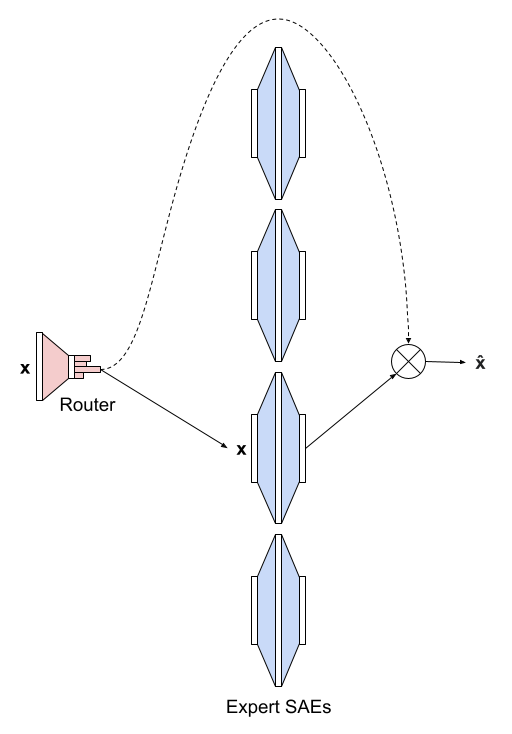
\includegraphics[width=3in]{fig/diagram.png}
\end{center}
\caption{\textbf{Switch Sparse Autoencoder Architecture.} The input activation passes through a router which sends it to the relevant expert SAE.}
\end{figure}

In total, the Switch Sparse Autoencoder contains \( 2Md + Nd + 2d \) parameters, whereas the TopK SAE has \( 2Md + d \) parameters. The additional \( Nd + d \) parameters we introduce through the router are an insignificant proportion of the total parameters because \( M \gg N \).

During the forward pass of a TopK SAE, \( Md \) parameters are used during the encoder forward pass, \( kd \) parameters are used during the decoder forward pass and \( d \) parameters are used for the bias, for a total of \( Md + kd + d \) parameters used. Since \( M \gg k \), the number of parameters used is dominated by \( Md \). During the forward pass of a Switch SAE, \( Nd \) parameters are used for the router, \( \frac{M}{N} d \) parameters are used during the encoder forward pass, \( kd \) parameters are used during the decoder forward pass and \( 2d \) parameters are used for the biases, for a total of \( \frac{M}{N} d + kd + Nd + 2d \) parameters used. Since the encoder forward pass takes up the majority of the compute, we effectively reduce the compute by a factor of \( N \). This approximation becomes better as we scale \( M \), which will be required to capture all the safety-relevant features of future superintelligent language models. Furthermore, the TopK SAE must compute and store \( M \) pre-activations. Due to the sparse router, the Switch SAE only needs to store \( \frac{M}{N} \) pre-activations, improving memory efficiency by a factor of \( N \) as well.

\subsection{Switch Sparse Autoencoder Training}
We train the Switch Sparse Autoencoder end-to-end. Weighting $E_i(\mathbf{x} - \mathbf{b}_{\text{pre}})$ by $p_i$ in the calculation of $\hat{\mathbf{x}}$ allows the router to be differentiable. We adopt many of the training strategies described in Bricken et al. and Gao et al. with a few exceptions. We initialize the rows (features) of $\mathbf{W}_{\text{enc}}^i$ to be parallel to the columns (features) of $\mathbf{W}_{\text{dec}}^i$ for all $i$. We initialize both $\mathbf{b}_{\text{pre}}$ and $\mathbf{b}_{\text{router}}$ to the geometric median of a batch of samples (but we do not tie $\mathbf{b}_{\text{pre}}$ and $\mathbf{b}_{\text{router}}$). We additionally normalize the decoder column vectors to unit-norm at initialization and after each gradient step. We remove gradient information parallel to the decoder feature directions. We set the learning rate based on the $\frac{1}{\sqrt{M}}$ scaling law from Gao et al. and linearly decay the learning rate over the last 20\% of training. We do not include neuron resampling (Bricken et al.), ghost grads (Jermyn et al.) or the AuxK loss (Gao et al.).

The ReLU SAE loss consists of a weighted combination of the reconstruction MSE and a L1 penalty on the latents to encourage sparsity. The TopK SAE directly enforces sparsity via its activation function and thus directly optimizes the reconstruction MSE. Following Fedus et al., we train our Switch SAEs using a weighted combination of the reconstruction MSE and an auxiliary loss which encourages the router to send an equal number of activations to each expert to reduce overhead. Empirically, we also find that the auxiliary loss improves reconstruction fidelity.

For a batch $\mathcal{B}$ with $T$ activations, we first compute vectors $\mathbf{f} \in \mathbb{R}^N$ and $\mathbf{P} \in \mathbb{R}^N$. $\mathbf{f}$ represents what proportion of activations are sent to each expert, while $\mathbf{P}$ represents what proportion of router probability is assigned to each expert. Formally,

\begin{equation}
f_i = \frac{1}{T} \sum_{\mathbf{x} \in \mathcal{B}} \1_{\{i^*(\mathbf{x}) = i\}} 
\end{equation}

\begin{equation}
P_i = \frac{1}{T} \sum_{\mathbf{x} \in \mathcal{B}} p_i(\mathbf{x})
\end{equation}

The auxiliary loss $\mathcal{L}_{\text{aux}}$ is then defined to be:

\begin{equation}
\mathcal{L}_{\text{aux}} = N \cdot \sum_{i=1}^N f_i \cdot P_i
\end{equation}

The auxiliary loss achieves its minimum when the expert distribution is uniform. We scale by $N$ so that $\mathcal{L}_{\text{aux}} = 1$ for a uniformly random router. The inclusion of $\mathbf{P}$ allows the loss to be differentiable.

The reconstruction loss $\mathcal{L}_{\text{recon}}$ is defined to be:

\begin{equation}
\mathcal{L}_{\text{recon}} = \frac{1}{T} \sum_{\mathbf{x} \in \mathcal{B}} \|\mathbf{x} - \hat{\mathbf{x}}\|_2^2
\end{equation}

Note that $\mathcal{L}_{\text{recon}} \propto d$. Let $\alpha$ represent a tunable load balancing hyperparameter. The total loss $\mathcal{L}_{\text{total}}$ is then defined to be:

\begin{equation}
\mathcal{L}_{\text{total}} = \mathcal{L}_{\text{recon}} + \alpha \cdot d \cdot \mathcal{L}_{\text{aux}}
\end{equation}

We optimize $\mathcal{L}_{\text{total}}$ using Adam ($\beta_1 = 0.9$, $\beta_2 = 0.999$).

\section{Results}

We train SAEs on the residual stream activations of GPT-2 small ($d = 768$). In this work, we follow Gao et al. and focus on layer 8. Using text data from OpenWebText, we train for 100K steps using a batch size of 8192, for a total of $\sim$820M tokens. We benchmark the Switch SAE against the ReLU SAE (Conerly et al.), the Gated SAE (Rajamanoharan et al.) and the TopK SAE (Gao et al.). We present results for two settings.

\begin{enumerate}
    \item Fixed Width: Each SAE is trained with $32 \cdot 768 = 24576$ features. We train Switch SAEs with 16, 32, 64 and 128 experts. Each expert of the Switch SAE with $N$ experts has $\frac{24576}{N}$ features. The Switch SAE performs roughly $N$ times fewer FLOPs per activation compared to the TopK SAE.
    
    \item FLOP-Matched: The ReLU, Gated and TopK SAEs are trained with $32 \cdot 768 = 24576$ features. We train Switch SAEs with 2, 4 and 8 experts. Each expert of the Switch SAE with $N$ experts has 24576 features, for a total of $24576 \cdot N$ features. The Switch SAE performs roughly the same number of FLOPs per activation compared to the TopK SAE.
\end{enumerate}

For a wide range of sparsity (L0) values, we report the reconstruction MSE and the proportion of cross-entropy loss recovered when the sparse autoencoder output is patched into the language model. A loss recovered value of 1 corresponds to a perfect reconstruction, while a loss recovered value of 0 corresponds to a zero-ablation.

\subsection{Fixed Width Results}

We train Switch SAEs with 16, 32, 64 and 128 experts (Figure 2, 3). The Switch SAEs consistently underperform compared to the TopK SAE in terms of MSE and loss recovered. The Switch SAE with 16 experts is a Pareto improvement compared to the Gated SAE in terms of both MSE and loss recovered, despite performing roughly 16x fewer FLOPs per activation. The Switch SAE with 32 experts is a Pareto improvement compared to the Gated SAE in terms of loss recovered. The Switch SAE with 64 experts is a Pareto improvement compared to the ReLU SAE in terms of both MSE and loss recovered. The Switch SAE with 128 experts is a Pareto improvement compared to the ReLU SAE in terms of loss recovered. The Switch SAE with 128 experts is a Pareto improvement compared to the ReLU SAE in terms of MSE, excluding when $k = 192$. The $k = 192$ scenario for the 128 expert Switch SAE is an extreme case: each expert SAE has $\frac{24576}{128} = 192$ features, meaning that the TopK activation is effectively irrelevant. When L0 is low, Switch SAEs perform particularly well. This suggests that the features that improve reconstruction fidelity the most for a given activation lie within the same cluster.

\begin{figure}[h]
\begin{center}
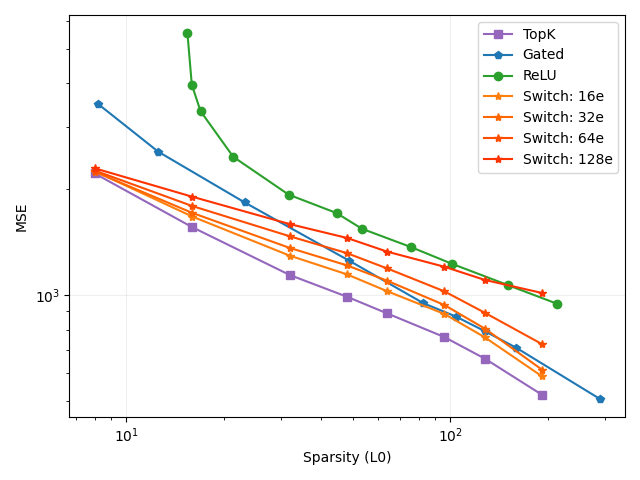
\includegraphics[width=4in]{fig/l0_mse.png}
\end{center}
\caption{\textbf{L0 vs. MSE for fixed width SAEs.} The 16 expert Switch SAE outperforms the Gated SAE. The 32 and 64 expert Switch SAEs outperform the ReLU SAE. The 128 expert Switch SAE outperforms the ReLU SAE excluding the extreme $k = 192$ setting.}
\end{figure}

\begin{figure}[h]
\begin{center}
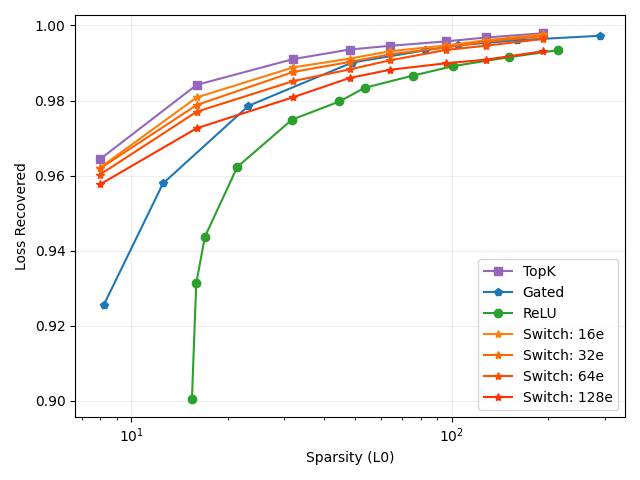
\includegraphics[width=4in]{fig/l0_lossrec.png}
\end{center}
\caption{\textbf{L0 vs. Loss Recovered for fixed width SAEs.} The 16 and 32 expert Switch SAEs outperform the Gated SAE. The 64 and 128 expert Switch SAEs outperform the ReLU SAE.}
\end{figure}

These results demonstrate that Switch SAEs can reduce the number of FLOPs per activation by up to 128x while still retaining the performance of a ReLU SAE. Switch SAEs can likely achieve greater acceleration on larger language models.

\subsection{FLOP-Matched Results}

We train Switch SAEs with 2, 4 and 8 experts (Figure 4, 5, 6). The Switch SAEs are a Pareto improvement over the TopK, Gated and ReLU SAEs in terms of both MSE and loss recovered. As we scale up the number of experts and represent more features, performance continues to increase while keeping computational costs and memory costs (from storing the pre-activations) roughly constant.



\begin{figure}[h]
\begin{center}
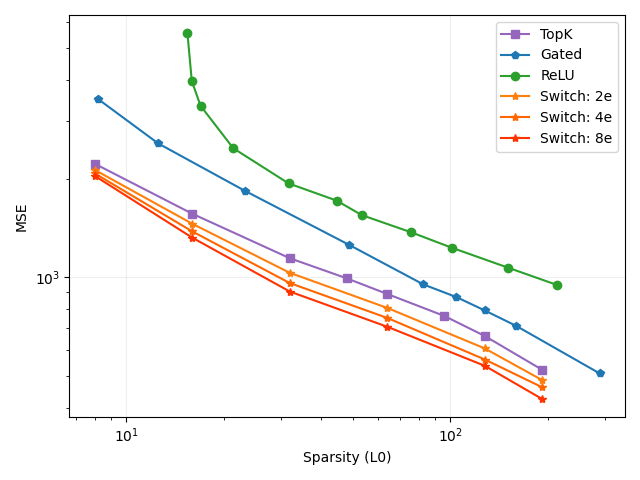
\includegraphics[width=4in]{fig/flopmatch_l0_mse.png}
\end{center}
\caption{\textbf{L0 vs. MSE for FLOP-matched SAEs.} The Switch SAEs consistently outperform the TopK, Gated and ReLU SAEs. Performance improves with a greater number of experts.}
\end{figure}

\begin{figure}[h]
\begin{center}
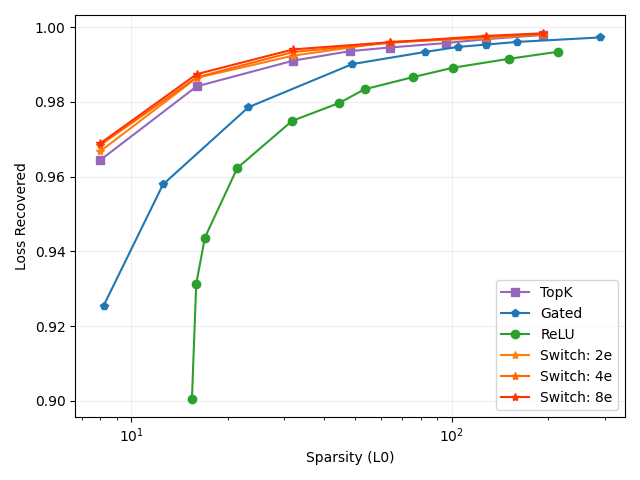
\includegraphics[width=4in]{fig/flopmatch_l0_lossrec.png}
\end{center}
\caption{\textbf{L0 vs. Loss Recovered for FLOP-matched SAEs.} The Switch SAEs consistently outperform the TopK, Gated and ReLU SAEs. Performance improves with a greater number of experts.}
\end{figure}

Fedus et al. find that their sparsely-activated Switch Transformer is significantly more sample-efficient compared to FLOP-matched, dense transformer variants. We similarly find that our Switch SAEs are 5x more sample-efficient compared to the FLOP-matched, TopK SAE baseline. Our Switch SAEs achieve the reconstruction MSE of a TopK SAE trained for 100K steps in less than 20K steps. This result is consistent across 2, 4 and 8 expert Switch SAEs.



\begin{figure}[h]
\begin{center}
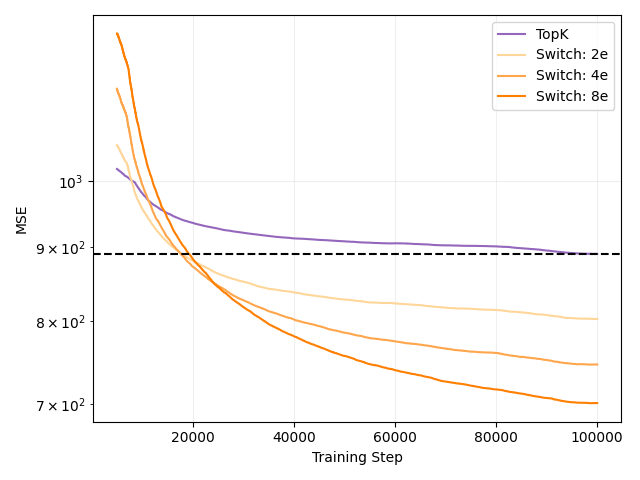
\includegraphics[width=4in]{fig/efficiency.png}
\end{center}
\caption{\textbf{Sample efficiency of Switch SAEs compared to the TopK SAE.} Switch SAEs achieve the same MSE as the TopK SAE in 5x fewer training steps.}
\end{figure}

Switch SAEs speed up training while capturing more features and keeping the number of FLOPs per activation fixed. Kaplan et al. similarly find that larger models are more sample efficient.



\section{Conclusion}
The diverse capabilities (e.g., trigonometry, 1960s history, TV show trivia) of frontier models suggest the presence of a huge number of features. Templeton et al. and Gao et al. make massive strides by successfully scaling sparse autoencoders to millions of features. Unfortunately, millions of features are not sufficient to capture all the relevant features of frontier models. Templeton et al. estimate that Claude 3 Sonnet may have billions of features, and Gao et al. empirically predict that future larger models will require more features to achieve the same reconstruction fidelity. If we are unable to train sufficiently wide SAEs, we may miss safety-crucial features such as those related to security vulnerabilities, deception and CBRN. Thus, further research must be done to improve the efficiency and scalability of SAE training. To monitor future superintelligent language models, we will likely need to perform SAE inference during the forward pass of the language model to detect safety-relevant features. Large-scale labs may be unwilling to perform this extra computation unless it is both computationally and memory efficient and does not dramatically slow down model inference. It is therefore crucial that we additionally improve the inference time of SAEs.

Thus far, the field has been bottlenecked by the encoder forward pass, the sole dense matrix multiplication involved in SAE training and inference. This work presents the first attempt to overcome the encoder forward pass bottleneck. Taking inspiration from Shazeer et al. and Fedus et al., we introduce the Switch Sparse Autoencoder, which replaces the standard large SAE with many smaller expert SAEs. The Switch Sparse Autoencoder leverages a trainable router that determines which expert is used, allowing us to scale the number of features without increasing the computational cost. When keeping the width of the SAE fixed, we find that we can reduce the number of FLOPs per activation by up to 128x while still maintaining a Pareto improvement over the ReLU SAE. When fixing the number of FLOPs per activation, we find that Switch SAEs train 5x faster and are a Pareto improvement over TopK, Gated and ReLU SAEs.

\subsection{Future Work}
This work is the first to combine Mixture-of-Experts with Sparse Autoencoders to improve the efficiency of dictionary learning. There are many potential avenues to expand upon this work.

\begin{itemize}
    \item We restrict our attention to combining the Switch layer (Fedus et al.) with the TopK SAE (Gao et al.). It is possible that combining the Switch layer with the ReLU SAE or the Gated SAE may have superior qualities.
    \item We require that every expert within a Switch SAE is homogeneous in terms of the number of features and the sparsity level. Future work could relax this constraint to allow for non-uniform feature cluster sizes and adaptive sparsity.
    \item Switch SAEs trained on larger language models may begin to suffer from dead latents. Future work could include a modified AuxK loss to prevent this.
    \item We restrict our attention to a single router. Future work could explore the possibility of further scaling the number of experts with hierarchical routers. Doing so may provide additional insight into feature splitting and geometry.
    \item Following Fedus et al., we route to a single expert SAE. It is possible that selecting several experts will improve performance. The computational cost will scale with the number of experts chosen.
    \item The routing network resembles the encoder of a sparse autoencoder. How do the feature directions of the routing network relate to the features of the corresponding expert SAEs?
    \item In this work, we train Switch SAEs on the residual stream, but future work could train Switch SAEs on the MLPs and attention heads.
\end{itemize}

\subsubsection*{Author Contributions}
xx.

\subsubsection*{Acknowledgments}
We used the dictionary learning repository to train our SAEs. We would like to thank Samuel Marks and Can Rager for advice on how to use the repository. We would also like to thank Jacob Goldman-Wetzler, Achyuta Rajaram, Michael Pearce, Gitanjali Rao, Satvik Golechha, Kola Ayonrinde, Rupali Bhati, Louis Jaburi, Vedang Lad, Adam Karvonen, Shiva Mudide, Sandy Tanwisuth, JP Rivera and Juan Gil for helpful discussions.


\bibliography{iclr2024_conference}
\bibliographystyle{iclr2024_conference}

\appendix
\section{Appendix}
xx.

\end{document}
